\section{Simulation}
\label{sec:simulation}

In this section, we investigate how to simulate future paths of the time series $y_t$. 
%We use this model to produce $K$ future values for the time serie $y_t$. 
Let $n$ be the total number of observations of $y_t$. We produce $S$ different paths with size $K$ for each. 
We have $n$ observations of $y_t$ and we want to produce . Given a vector of explanatory variables $x_t$, let $q_t^\alpha$ be given by the following linear model:
\begin{equation}
q_t^\alpha = \beta_0^\alpha +  x_t^T \beta^\alpha + \varepsilon_t,
\label{eq:fun-quantile}
\end{equation}
where $\beta^\alpha$ is a vector of coefficients for the explanatory variables. The variables chosen to compose $x_t$ can be either exogenous variables, autoregressive components of $y_t$ or both. As the distribution of $\varepsilon_t$ is unknown, we have to use a nonparametric approach in order to estimate its one-step ahead density.

The coefficients $\beta_0^\alpha$ and $\beta^\alpha$ are the solution of the minimization problem given in the problem defined in (\ref{eq:non-crossing-quantiles1})-(\ref{eq:non-crossing-constraint}), reproduced here for convenience:
\begin{eqnarray}
\label{eq:non-crossing-quantiles1-sim}
\min_{q,\varepsilon_{t,\alpha}^{+}, \varepsilon_{t,\alpha}^{-}} &  \sum_{\alpha \in A} \sum_{t \in T}\left(\alpha \varepsilon_{t,\alpha}^{+}+(1-\alpha)\varepsilon_{t,\alpha}^{-}\right) &  \\
\mbox{s.t. } & \varepsilon_{t,\alpha}^{+}-\varepsilon_{t,\alpha}^{-}=y_{t}-q^\alpha(x_{t}), & \qquad\forall t \in T_\tau,\forall \alpha \in A,\\
& \varepsilon_{t,\alpha}^+,\varepsilon_{t,\alpha}^- \geq 0, & \qquad\forall t \in T_\tau,\forall \alpha \in A,\\\label{eq:non-crossing-constraint-sim}
& q_t^{\alpha} \leq q_t^{\alpha'}, & \qquad \forall t \in T_\tau, \forall \alpha, \alpha' \in A, \alpha < \alpha', 
\end{eqnarray}

To produce $S$ different paths of $\{ \hat{y}_t \}_{t=n+1}^{n+K}$, we use the following procedure:

\noindent\rule{\textwidth}{3pt}

Procedure for simulating $S$ scenarios of $y_t$

\noindent\rule{\textwidth}{1pt}

\begin{enumerate}
	
\item At first, let $\tau = n + 1$.

\item In any given period $\tau$, for a sequence $0 < \alpha_1 < \alpha_2 < \dots < \alpha_Q < 1$, we use the problem defined on  (\ref{eq:non-crossing-quantiles1})-(\ref{eq:non-crossing-constraint}) to predict quantiles 
 $q^{\alpha_1}_{t} \leq q^{\alpha_2}_{t} \leq \dots \leq q^{\alpha_Q}_{t}$.
Note that $x_{\tau}$ is supposed to be known at time $\tau$. In the presence of exogenous variables that are unknown, it is advisable to incorporate its uncertainty by considering different scenarios. In each scenario, though, $x_{\tau}$ must be considered fully known. 
 
\item Let $F_{y_{\tau}}$ be the estimated distribution function of ${y}_{\tau}$. 
The process of fitting $\hat{F}_{y_{\tau}}$ is by mapping every $\alpha_i$ with its estimated quantile $\hat{q}^{\alpha_i}$. A problem arises for the distribution extremities, because when $\alpha = 0$ or $\alpha = 1$, the optimization problem becomes unbounded.
In order to find good estimates for $y_{\tau}$ when $F_{y_{\tau}}$ approaches 0 or 1, we can either use a kernel smoothing function, splines, linear approximation, or any other method. 
\textbf{This will be developed later.}
When this sequence of chosen $\alpha_i$ is thin enough, we can approximate well the distribution function of $y_{\tau}$, as is shown in Figure \ref{fig:grafico-quantis}. 
Thus, the distribution found for $\hat{y}_{\tau}$ is nonparametric, as no previous assumptions are made about its shape, and its form is fully recovered by the data we have.

\begin{figure}[h]
\centering
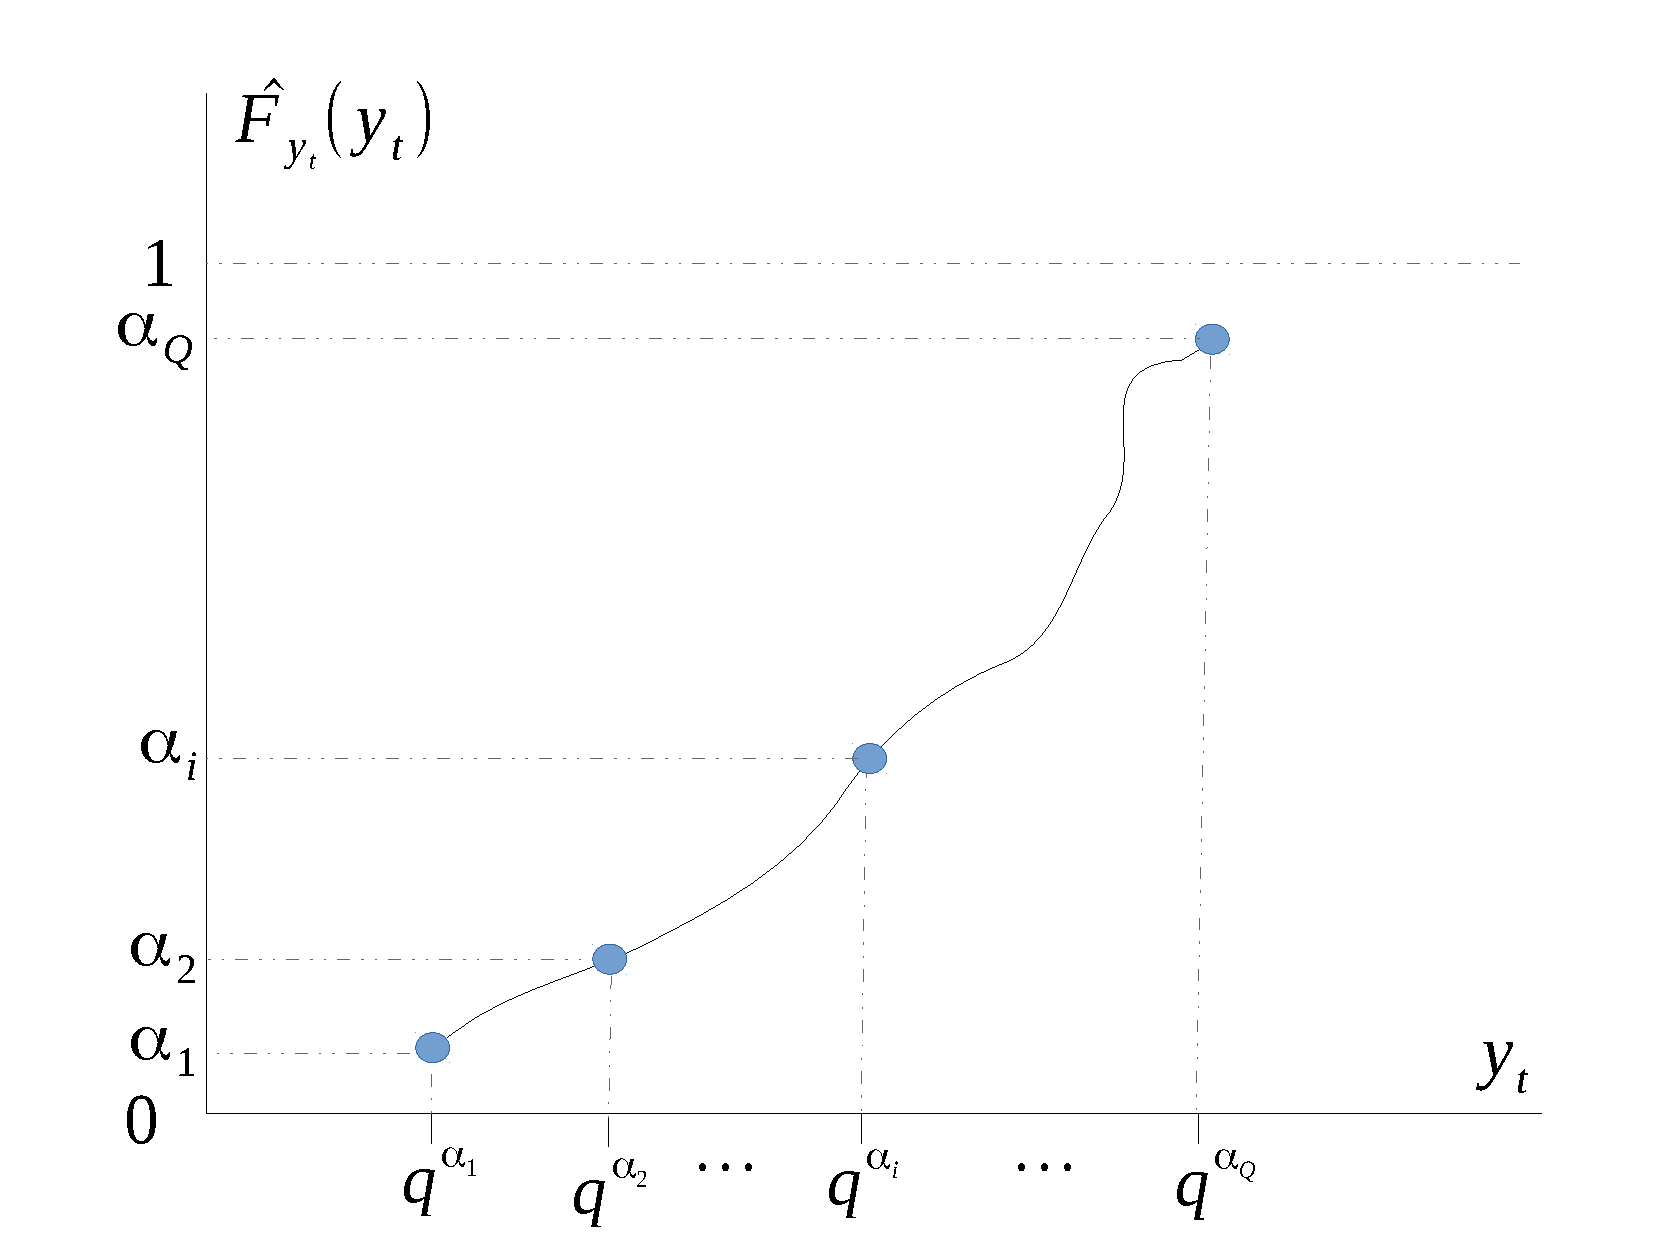
\includegraphics[width=0.7\linewidth]{./Figuras/grafico-quantis}
\caption{Fitting a distribution function from quantile estimations}
\label{fig:grafico-quantis}
\end{figure}


\item Once we have a distribution for $y_{n+1}$, we can generate $S$ different simulated values, drawn from the distribution $\hat{F}_{y_{n+1}}$ found by doing steps 2 and 3. 
Let $X$ be a random variable with uniform distribution over the interval $[0,1]$. By using results from the Probability Integral Transform, we know that the random variable $F^{-1}_{y_{n+1}}(X)$ has the same distribution as $y_{n+1}$. So, by drawing a sample of size $S$ from $X$ and applying the inverse function of $F_{y_{n+1}}$, we have our sample of size $K$ for $y_{n+1}$.

\item Each one of the $S$ different values for $y_{n+1}$ will be the starting point of a different path. Now, for each $\tau \in [n+2,n+K]$ and $s \in S$, we have to estimate the quantiles $q_{\tau,s}^{\alpha_i}$ and find a distribution function for $\hat{F}_{y_{\tau,s}}$ just like it was done on steps 2 and 3.
Note that when $\tau > n+2$, every estimate will be scenario dependent, hence there will be $S$ distribution functions estimated for each period $\tau$. From now on, in each path just one new value will be drawn randomly from the one-step ahead distribution function - as opposed to what was carried on step 3, when $S$ values were simulated. As there will be $S$ distribution functions - one for each path, in each period $\tau$ it will be produced exact $S$ values for $y_\tau$, one for its own path. Repeating this step until all values of $\tau$ and $s$ are simulated will give us the full simulations that we are looking for.
\end{enumerate}


\noindent\rule{\textwidth}{1pt}